\documentclass[finnish, 12pt, a4paper, elec, latin1, utf8, online]{aaltothesis}
%\documentclass[finnish, 12pt, a4paper, elec, utf8, a-1b]{aaltothesis}
%\documentclass[finnish, 12pt, a4paper, elec, dvips, online]{aaltothesis}
%\documentclass[english, 12pt, a4paper, elec, utf8, a-1b, online]{aaltothesis}
%\documentclass[english, 12pt, a4paper, elec, utf8, a-1b]{aaltothesis}
%\documentclass[english, 12pt, a4paper, elec, dvips, online]{aaltothesis}
%\usepackage[a-1a]{pdfx}
%\usepackage[T1]{fontenc}
%\usepackage{fontspec}

\usepackage{graphicx}
\usepackage{epstopdf}
\usepackage{datetime} 
\usepackage{amsfonts,amssymb,amsbsy}
\usepackage{csquotes}
\usepackage[natbib=true,style=numeric-comp,sorting=none]{biblatex}
\addbibresource{sources.bib}

\hyphenpenalty=100000
\setlength{\parindent}{0em}
\setlength{\parskip}{1em}

\degreeprogram{Elektroniikka ja sähkötekniikka}
\major{Elektroniikka ja sähkötekniikka}
\code{ELEC3013}
\univdegree{BSc}
\thesisauthor{Aarni Halinen}
\pagenumbering{gobble}
\thesistitle{IoT-soveltuva tiedonlähetys LTE-järjestelmissä}
\place{Espoo}
\date{24.4.2018}
\supervisor{TkT Markus Turunen}
\advisor{TkT Kalle Ruttik}
\uselogo{aaltoRed}{''}

%% Suomenkielinen tiivistelmä:
\keywords{IoT, LTE, M2M, MulteFire}
\thesisabstract{
Esineiden internetin (IoT) myötä internetiin kytkettyjen laitteiden määrä kasvaa räjähdysmäisesti. IoT-laitteiden kommunikaatio vaatii verkolta mahdollisuutta vähävirtaiseen tiedonsiirtoon, laajaa maantieteellistä peittoa ja alhaisia kustannuksia. LTE-standardiin on tehty viime aikoina lukuisia päivityksiä, jotka mahdollistavat ihmisten väliseen kommunikaation tarkoitetun verkon käytön myös koneille. Kirjallisuustutkimuksen tavoitteena oli selvittää, miten LTE-järjestelmää on kehitetty viimeisimmissä standardin julkaisuissa tukemaan paremmin esineiden internetin tarpeita. \textit{Release 13}:ssa esiteltiin kapeakaistainen esineiden internet (NB-IoT), joka mahdollistaa tuen erittäin yksinkertaisille IoT-laitteille. Myöhemmissä \textit{Release 14} ja \textit{Release 15} julkaisuissa tekniikkaa kehitettiin edelleen, minkä lisäksi LTE-verkkojen kapasiteetin parantamiseksi standardia on kehitetty toimimaan lisensoimattomalla radiospektrillä. Lisensoimattomalla spektrillä toimii myös LTE-standardiin perustuva MulteFire-teknologia.
}

\copyrighttext{Copyright \noexpand\copyright\ \number\year\ \ThesisAuthor}
{Copyright \copyright{} \number\year{} \ThesisAuthor}

%% Voit estää LaTeXia kirjoittamasta xmpdata-tiedostoon (sisältää pdf-tiedostoon
%% kirjoitettavaa metadataa) asettamalla writexmpdatafile lipun arvoksi 'false'.
%% Tämä mahdollistaa sen, että voit kirjoittaa metadataa suoraan oikeassa
%% muodossa tiedostoon opinnaytepohja.xmpdata.
%%
%\setboolean{writexmpdatafile}{false}
%%

\begin{document}
\makecoverpage{}
\makecopyrightpage{}

\begin{abstractpage}[finnish]
\abstracttext{}
\end{abstractpage}
\newpage

%% Englanninkielinen tiivistelmä:
\thesistitle{IoT capable data transfer in LTE systems}
\supervisor{D.Sc. (Tech.) Markus Turunen}
\advisor{D.Sc. (Tech.) Kalle Ruttik}
\degreeprogram{Electronics and Electrical Engineering}
\major{Electronics and Electrical Engineering}
%\keywords{IoT, LTE, M2M, MulteFire}
\begin{abstractpage}[english]
With Internet of Things, the number of devices connected to the Internet grows massively. Communication of the devices require ability for low power consumption, large coverage and low device cost from the network. Recently, a number of new releases have been made to the LTE standard, enabling Machine-to-machine communication in the network. The main objective of this research was to find out how the LTE standard has developed in the most recent releases to meet the requirements of M2M. \textit{Release 13} introduced Narrowband IoT that allows support for low complexity IoT devices. The technology was further developed in subsequent releases. In addition, LTE standard was developed to work within unlicensed spectrum to improve the capacity of the network. Also MulteFire, a new technology based on the LTE, functions within the unlicensed spectrum.
\end{abstractpage}

\newpage

\mysection{Esipuhe}

Haluan kiittää ohjaajaani Kalle Ruttikia tuesta ja hyvästä työn ohjauksesta. Haluan myös kiittää Sofia Suutarista laadukkaasta opponoinnista ja syvästä kiinnostuksesta työni aihetta kohtaan. Lisäksi haluan kiittää toista kandipienryhmäläistäni Jan Tuomea ja perhettäni tuesta, palautteesta ja oikoluvussa auttamisesta. \\

\vspace{5cm}
Otaniemi, 24.4.2018

\vspace{5mm}
{\hfill \ThesisAuthor \hspace{1cm}}
\newpage


\thesistableofcontents

\mysection{Symbolit ja lyhenteet}
\subsection*{Lyhenteet}
%\subsection*{Abbreviations}
\begin{tabular}{ll}
3GPP & 3rd Generation Partnership Project \\
5G & 5th Generation \\
5G-NR & 5G New Radio \\
AD & Analog-to-digital \\
ATIS & Alliance for Telecommunications Industry Solution \\
CCSA & China Communications Standards Association \\
CID & Cell-ID \\
CSMA & Carrier-sense multiple access \\
D2D & Device-to-Device \\
DRX & Discontinuous reception  \\
eLAA & enhanced LAA \\
eMBB & enhanced Mobile Broadband \\
eMTC & enhanced Machine-Type Communication \\
ETSI & European Telecommunications Standards Institute \\
FDD & Frequency-Division Duplex \\
%FDMA & Frequency-Division Multiple Access \\
GSM & Global System for Mobile Communications \\
H2H & Human-To-Human \\
HARQ & Hybrid automatic repeat request \\
IoT & Internet of Things \\
IP & Internet Protocol \\
ITS & Intelligent Transport Systems \\
LAA & License Assisted Access \\
LBT & Listen-before-talk \\
LPWA & Low-Power Wide-Area \\
LTE & Long-Term Evolution \\
LTE-A & Long-Term Evolution Advanced \\
LTE-M & LTE for M2M \\
LTE-U & LTE Unlicensed \\
LWA & LTE-WLAN aggregation \\
M2M & Machine-to-Machine \\
MIB & Master Information Block \\
MIMO & Multiple-Input and Multiple-Output \\
mMTC & massive Machine Type Communications \\
MTC-IWF & Multicast Traffic Channel Interworking Function \\
NB-IOT & NarrowBand Internet of Things \\
NFC & Near-field Communication \\
NPBCH & NarrowBand Physical Broadcast Channel \\
NPDCCH & NarrowBand Physical Downlink Control Channel \\
NPDSCH & NarrowBand Physical Downlink Shared Channel \\
NPRACH & NarrowBand Physical Random Access Channel \\
NPUSCH & NarrowBand Physical Uplink Shared Channel \\
NPRS & NarrowBand Positioning Reference Signal \\
NPSS & NarrowBand Primary Synchronization Signal \\
NSSS & NarrowBand Secondary Synchronization Signal \\
\end{tabular}
\clearpage
\begin{tabular}{ll}
OFDM & Orthogonal Frequency-Division Multiplexing \\
OFDMA & Orthogonal Frequency-Division Multiple Access \\
OMA & Open Mobile Alliance \\
OTDOA & Observed Time Difference Of Arrival \\
%PBCH & Physical Broadcast Channel \\
PCFICH & Physical Control Format Indicator Channel \\
PDCCH & Physical Downlink Control Channel \\
PDSCH & Physical Downlink Shared Channel \\
PHICH & Physical Hybrid ARQ Indicator Channel \\
PMCH & Physical Multicast Channel \\
PRACH & Physical Random Access Channel \\
%PUCCH & Physical Uplink Control Channel \\
%PUSCH & Physical Uplink Shared Channel \\
PRB & Physical Resource Block \\
PSDN & Public Switched Data Network \\
RA & Random Access \\
RAN & Radio Access Network \\
RFID & Radio-frequency identification \\
SAE & System Architecture Evolution \\
SC-FDMA & Single-carrier Frequency division multiple access\\
SIB & System Information Block \\
SIM & Subscriber identity module \\
UMTS & Universal Mobile Terrestrial System \\
TAU & Tracking Area Update \\
TBS & Transport Block Size \\
TDD & Time-Division Duplex \\
ToA & Time of arrival \\
URLLC & Ultra Reliable Low Latency Communications \\
QAM & Quadrature Amplitude Modulation \\
QPSK & Quadrature Phase Shift Keying \\
\end{tabular}

%% \clearpage on melkein samanlainen kuin newpage, mutta 
%% flushaa myös LaTeX:n floatit 
\cleardoublepage

\section{Johdanto}
\pagenumbering{arabic}
%\section{Introduction}

Esineiden internetillä (IoT) tarkoitetaan laitteiden välistä yhteyttä ja tiedonsiirtoa internetin avulla. Se mahdollistaa uudenlaisia palveluita muun muassa turvallisuuden, laitteiden huollon ja päivittämisen sekä älykkäiden verkkojen saralla. Esineiden internetin myötä verkkoon kytkettyjen laitteiden määrä kasvaa räjähdysmäisesti 2020-luvulle mentäessä. Arviolta 50 miljardia laitetta on kytketty internetiin vuonna 2020 \cite{ratasuk2016nb}.

Verkon liikenteestä suuren osan tulevaisuudessa muodostavat erilaiset sensorit, jotka viestivät palvelimien ja muiden IoT-laitteiden kanssa. Toimiva tuki laitteiden väliselle kommunikaatiolle (M2M) on välttämätön edellytys esineiden internetin muodostumiselle \cite{nokiawhitepaper}. M2M-kommunikaatio voi tapahtua verkon yli tai suoraan laitteelta toiselle laitteelle (D2D). M2M-kommunikaation mahdollistamia palveluita ovat muun muassa huoltotarvetta tarkkailevat sensorit ja erilaiset paikannuslaitteet. Tällaisten IoT-laitteiden tiedonsiirto koostuu pääosin pienistä datalähetyksistä, joita lähetetään varsin harvoin. Laitteiden toiminnalle on tärkeää, että laitteen ja verkon välinen kommunikaatio ei kuluta resursseja turhaan. Kommunikaatio ei myöskään saa rasittaa verkkoa liikaa.

3rd Generation Partnership Project -organisaation (3GPP) standardoimaan Long Term Evolution -järjestelmään (LTE) on muutaman viime vuoden aikana tehty useita päivityksiä tukemaan IoT-laitteille sopivaa, pienen tehonkulutuksen kommunikaatiota. LTE:n \textit{Release 12} \cite{release12} esitteli LTE-M teknologian keskisuuria tiedonsiirtonopeuksia ja liikkuvia IoT-laitteita varten \cite{ratasuk2016overview}. \textit{Release 13}:ssa \cite{release13} esiteltiin kapeakaistainen esineiden internet (NB-IoT) matalan kompleksisuuden laitteille sekä paranneltiin LTE-M-teknologiaa. NB-IoT:n on tarkoitus tarjota halpoja laitteistototeutuksia, yli 10 vuoden akunkestoa IoT-laitteille, sekä mahdollisuus kytkeä yli 52 000 laitetta samanaikaisesti samalle kanavalle \cite{nokiawhitepaper}. Koska NB-IoT on kehitelty jo olemassa olevia LTE-toteutuksia hyödyntäväksi, on se myös mahdollista ottaa käyttöön vähäisin kustannuksin.

Tässä työssä tutkitaan, miten LTE-järjestelmiä on muokattu tukemaan IoT-laitteiden datalähetyksiä. Tutkimus toteutetaan kirjallisuustutkimuksena. Toisessa luvussa käsitellään M2M-kommunikaatiota ja kartoitetaan IoT-laitteiden asettamia vaatimuksia verkoille. Kolmannessa luvussa käsitellään LTE-järjestelmän standardointia ja esineiden internetille tärkeimpiä LTE-standardin muutoksia. Neljännessä luvussa tutustutaan uusimpaan \textit{Release 14} -julkaisuun ja kehitteillä olevaan \textit{Release 15} -julkaisuun IoT-laitteiden näkökulmasta. Tämän lisäksi luvussa tutustutaan, miten LTE:n ja siihen perustuvassa MulteFire-järjestelmän kehitystyössä on alettu hyödyntää lisensoimatonta radiospektriä.

\clearpage
\section{M2M-kommunikaatio}

\subsection{Esineiden internet}

Esineiden internet -termi kehitettiin vuonna 1999 kuvaamaan RFID-tunnisteilla varustettujen laitteiden globaalia verkkoa \cite{sundmaeker2010vision}. Termi on nykyään laajentunut määrittelemään esineiden muodostama verkkoa, jossa laitteet keräävät ja lähettävät tietoa toisilleen \cite{atzori2010internet}. Verkon esineet voivat olla kaikkea suurista teollisuuden laitteista sensoreihin tai puettaviin tietokoneisiin, kuten älykelloihin. Autonomisesti toisilleen viestivät laitteet mahdollistavat tehokkaampia laitteita ja parempia käyttäjäkokemuksia. Tämä laitteiden välinen kommunikaatio, eli niin sanottu Machine-to-machine -kommunikaatio (M2M), on edellytys esineiden internetin muodostumiselle \cite{nokiawhitepaper}.

%\begin {figure}[h!]
%    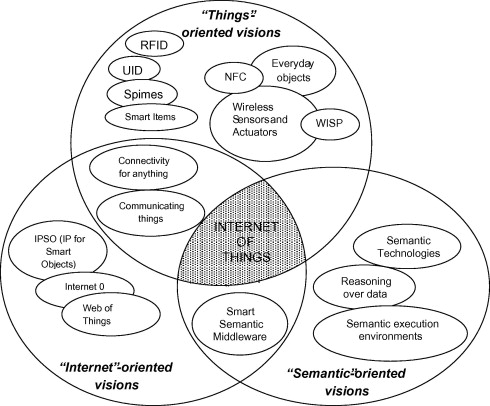
\includegraphics[width=\linewidth]{IoT.jpg}
%    \caption{Esineiden internet eri näkökulmista. \cite{atzori2010internet}}
%    \label{fig:IoT}
%\end {figure}

%Esineiden internet voidaan jakaa 

Esineiden internetin päätelaitteiden tuottama verkkoliikenne voidaan jakaa kiinteän ja lyhyen kantaman liikenteeseen, mobiiliverkkojen ja LPWA-verkkojen kautta kulkevaan liikenteeseen \cite{nokiawhitepaper, harmaala}. Päätelaitteista suurin osa kommunikoi kiinteän ja lyhyen kantaman yhteyksiä hyväksi käyttäen \cite{nokiawhitepaper}. Tällaisia yhteyksiä ovat muun muassa Bluetooth ja NFC. Kuitenkin noin 7 miljardia laitetta kommunikoi käyttäen perinteisiä mobiili- ja LPWA-verkkoja \cite{nokiawhitepaper}.

LPWA-verkot on jaettu 3GPP:n standardoinnin ulkopuolisiin, usein lisensoimattomalla radiospektrillä toimiviin verkkoihin, kuten SigFox ja LoRa, sekä 3GPP:n standardoimiin mobiiliverkkoihin perustuviin LPWA-verkkoihin \cite{nokiawhitepaper}. Nämä verkot toimivat useimmiten lisensoidulla radiospektrillä. 3GPP:n standardoimia teknologioita ovat \textit{Release 12}:ssa julkaistu LTE-M sekä \textit{Release 13}:n esittelemä NB-IoT. Tässä luvussa esitellään mobiiliverkkoa hyödyntävien IoT-laitteiden asettamia haasteita ja edellytyksiä LTE-verkolle.

\subsection{M2M-kommunikaation edellytykset LPWA-verkoille}

LPWA-verkot ovat tärkeässä roolissa turvallisten, pienitehoisten, pitkän kantaman ja alhaisen hinnan laitteiden yhdistämisessä osaksi esineiden internetiä \cite{gsmawhitepaper}. Tällaisia palveluja ovat muun muassa logistiikkaan, älykkäisiin kaupunkeihin, maanviljelyyn ja ympäristöön sekä infrastruktuuriin liittyvät palvelut. Nämä palvelut tarvitsevat useimmiten laajaa kattavaa verkkoa, kuuluvuutta myös sisätiloissa, ja ne toimivat ilman verkkovirtaa \cite{gsmawhitepaper}. Jotta palveluiden M2M-kommunikaatio olisi mahdollista ja taloudellisesti järkevää, LPWA-verkon tulee mahdollistaa päätelaitteille pitkä akunkesto ja laaja maantieteellinen peitto. Samalla niiden täytyy tukea suurta laitemäärää ja pitää päätelaitteiden laitteisto- ja kehityskustannukset matalina.

Akunkeston pidentämistä voidaan pitää merkittävimpänä haasteena verkolle, sillä päätelaite voi olla vaikeakulkuisessa paikassa tai jatkuvassa liikkeessä, minkä vuoksi akun vaihtaminen on työlästä ja kallista \cite{nokiawhitepaper}. Kestävä akku mahdollistaa myös uusien palvelujen kehittämisen. Päivittäin dataa keräävän ja pieninä paketteina lähettävän laitteen akun pitäisi kestää alalla vallitsevan käsityksen mukaan vähintään 10 vuotta.

Verkon kattavuus on tärkeää monille IoT-laitteille, jotka saattavat sijaita rakennusten kellareissa tai muilla verkon katvealueilla \cite{nokiawhitepaper}. Esimerkiksi hissit ja liukuhihnat voivat toimia sisätiloissa paksujen seinien peittäminä. Heikompaa signaalin voimakkuutta sietävät päätelaitteet, suunnatut antennit ja päätelaitteiden kommunikaation ketjutus ratkaisevat osaltaan kattavuuden parantamisen \cite{diaz20163gpp}.

Esineiden internetin myötä verkkoon kytkettyjen laitteiden määrä kasvaa, ja vuoteen 2025 mennessä LPWA-verkkoihin on kytkettynä noin 7 miljardia IoT-laitetta, mikä vastaa nykyhetken globaalia mobiililiittymien tilaajamäärää \cite{nokiawhitepaper}. Lisääntynyt liikenne voi ruuhkauttaa verkkoa, mikä hidastaa sekä koneiden että ihmisten välistä liikennettä \cite{diaz20163gpp}. Kaikki verkon laitteet eivät myöskään jakaudu tasaisesti solujen välille, joten yksittäisen verkon solun täytyy pystyä tukemaan hyvin suurta laitemäärää \cite{nokiawhitepaper}. Jo yhden solun ylikuormitus heikentää myös muiden solujen suorituskykyä.

Alhaiset päätelaitekustannukset ovat tärkeä osa LPWA-verkon houkuttelevuutta. IoT-palveluntarjoajille on tärkeää, että LPWA-verkkoon kyetään yhdistämään matalan kompleksisuuden laitteilla, sillä palveluntarjoajien liiketoiminta perustuu usein lukuisten sensorien keräämään dataan. Tavoitteena alalla on alle viiden dollarin hinta moduulille \cite{nokiawhitepaper}. Laitekustannusten lisäksi verkkoon yhdistämisen tulee olla mahdollisimman edullista, jotta palveluiden pariin on mahdollista houkutella riittävästi alhaisista hinnoista kiinnostuneita asiakkaita \cite{harmaala}. Lisäksi LPWA-verkon pystyttäminen tulee pitää hinnaltaan alhaisena. LTE-järjestelmässä NB-IoT- tai LTE-M-verkko kyetään toteuttamaan olemassa olevalle laitteistolle ohjelmistopäivityksenä, joten verkolle ei tarvita laitteistohankintoja \cite{nokiawhitepaper}.

\clearpage
\section{LTE-järjestelmän standardointi}

\subsection{Standardointiprosessi}

LTE-standardin kehityksestä ovat yhteistyössä vastuussa 3rd Generation Partnership Project (3GPP), European Telecommunications Standards Institute (ETSI), Open Mobile Alliance (OMA), China Communications Standards Association (CCSA) ja Alliance for Telecommunications Industry Solution (ATIS) \cite{ghavimi2015m2m}. Edellä mainituista instituutioista 3GPP on vastuussa M2M-kommunikaation sulauttamisesta osaksi mobiiliverkkoja, kun taas vastaavasti ETSI:n vastuulla on M2M-kommunikaation palveluarkkitehtuuri. 

3GPP:n tavoitteena kehitystyössä on muokata LTE-järjestelmän ydinverkkoa (SAE) tukemaan paremmin M2M-kommunikaatiota \cite{ghavimi2015m2m}. Ensimmäiset M2M-kommunikaation mahdollistavat järjestelmäparannukset julkaistiin \textit{Release 10}:ssä, kun verkon rungoksi valittiin Universal Mobile Terrestrial System (UMTS) ja LTE-Advanced -verkot (LTE-A). \textit{Release 10} -standardin tavoitteena M2M-kommunikaation osalta oli optimoida järjestelmän kykyä käsitellä M2M-signaloinnin ruuhkasta ja verkon ylikuormittumisesta aiheutuvia ongelmia. \textit{Release 10}:n jälkeen 3GPP:n kehitysprosessin pääpaino on siirtynyt standardoidun järjestelmäverkon arkkitehtuuriparannuksien tutkimiseen. Tutkimuksen tavoitteena on tunnistaa tarvittavat verkon kehityskohteet ja M2M-palveluiden kannalta olennaisimmat tekijät, jotta verkkoinfrastruktuuri pystyisi tukemaan mahdollisimman suurta yhtäaikaista päätelaitteiden määrää.

\subsection{LTE-järjestelmän kehysrakenne}

\textit{Release 8}:ssa on LTE-järjestelmille määritelty kaksi kehysrakennetta, joiden avulla LTE-järjestelmät ja liikenne tukiasemien ja päätelaitteiden välillä pysyy synkronoituna. Tyypin yksi (kuva \ref{fig:type1}) kehysrakenne tukee taajuusjakoista kaksisuuntaisuutta (FDD), kun taas tyypin kaksi (kuva \ref{fig:type2}) kehysrakenne on aikajakoista kaksisuuntaisuutta (TDD) varten \cite{ETSIts36211}. Molempien kehysrakenteiden lataus- ja lähetyslinkkien aikaintervallit ilmaistaan perusaikayksikön \begin{equation}
    T_s = \frac{1}{1500 \cdot 2048}
\end{equation}
monikertoina. Täten yksi radiokehys on kestoltaan
\begin{equation}
    T_f = 307200 \cdot T_s = 10 \textrm{ ms.}
\end{equation}

Tyypin 1 radiokehys on soveltuva sekä vuoro- että kaksisuuntaiseen liikenteeseen (half-duplex, full duplex) \cite{ETSIts36211}. Jokainen radiokehys on jaettu 20:een, \begin{equation}
    T_{slot} = \frac{T_f}{20} = 0,5 \textrm{ ms}
\end{equation}
pituisiin osiin, jotka on numeroitu 0--19. Alikehyksellä tarkoitetaan kahta peräkkäistä radiokehyksen osaa. Jokaisella 10 millisekunnin radiokehyksellä on 10 alikehystä varattu lähetyslinkille ja toiset 10 latauslinkille. Linkit on erotettu toisistaan taajuustasossa, minkä vuoksi vuorosuuntaisessa liikenteessä päätelaitteet eivät pysty lähettämään ja vastaanottamaan samanaikaisesti.

\begin{figure}[h!]
    \centering
    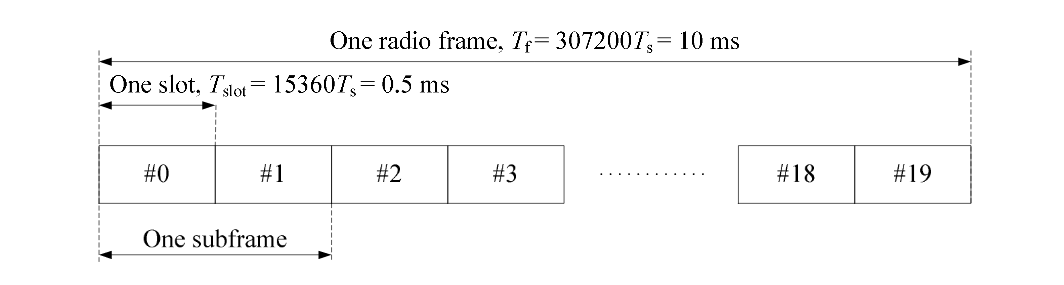
\includegraphics[width=\linewidth]{Images/radioframe1.png}
    \caption{Tyypin yksi LTE-radiokehyksen rakenne \cite{ETSIts36211}.}
    \label{fig:type1}
\end{figure}

Tyypin 2 radiokehys on käytössä aikajakoiselle liikenteelle \cite{ETSIts36211}. Sen 10 millisekunnin kehys on jaettu kahteen 5 millisekunnin puolikehykseen, jotka on puolestaan jaettu viiteen, yhden millisekunnin pituiseen, alikehykseen.

\begin{figure}[h!]
    \centering
    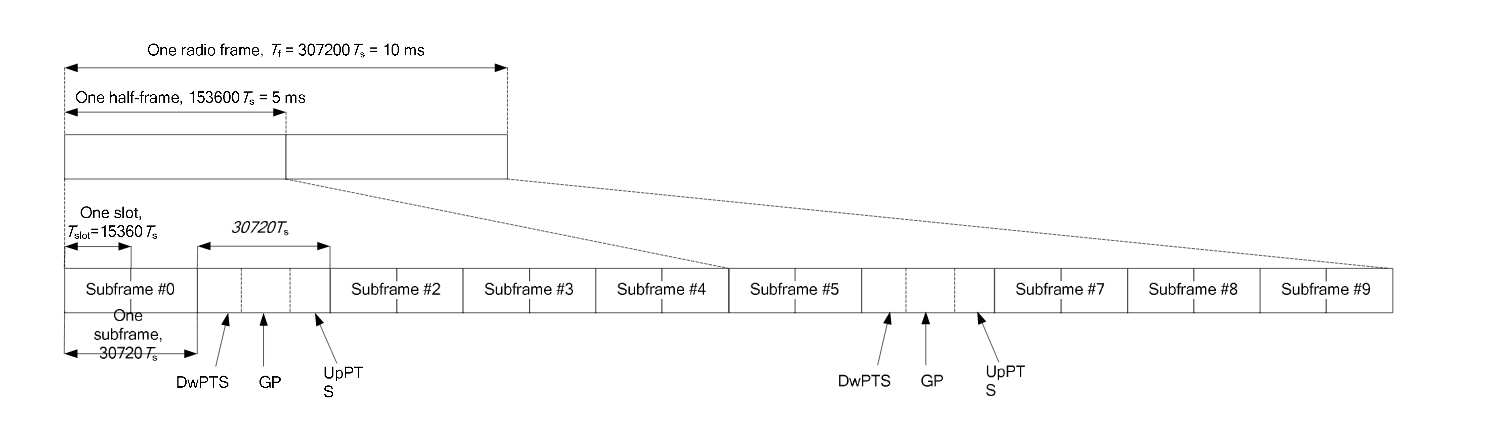
\includegraphics[width=\linewidth]{Images/radioframe2.png}
    \caption{Tyypin kaksi LTE-radiokehyksen rakenne \cite{ETSIts36211}.}
    \label{fig:type2}
\end{figure}

LTE-järjestelmän lähettämät signaalit voidaan esittää kuvan \ref{fig:PRB} mukaisella resurssilohkolla. Lohkon pienimpiä aika-taajuusykiskköjä kutsutaan resurssielementeiksi, ja niistä jokainen on tunnistettavissa indeksiparin $(k,l)$
\begin{equation}
    k = 0, ..., N^{DL}_{RB}N^{RB}_{SC} -1
\end{equation} 
ja
\begin{equation}
    l = 0, ..., N^{DL}_{symb} -1
\end{equation}
avulla. Resurssielementti jossain tietyssä antenniportissa $p$ voidaan ilmaista kompleksiluvulla $a_{k,l}^{(p)}$. Elementit, joita ei käytetä fyysisen kanavan tai signaalin lähettämiseen, tulee olla asetettuina nollaksi. \cite{ETSIts36211}

\begin{figure}[h!]
    \centering
    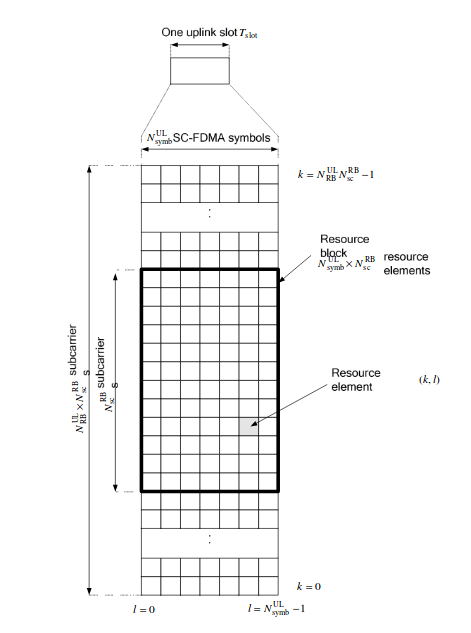
\includegraphics[scale=0.5]{Images/ResourceBlock.png}
    \caption{LTE-järjestelmän resurssilohko (PRB) radiokehyksessä \cite{ETSIts36211}.}
    \label{fig:PRB}
\end{figure}

\subsection{LTE ja M2M}

M2M-sovellukset eroavat merkittävästi H2H-tyyppisestä kommunikaatiosta, minkä takia alunperin H2H-kommunikaatioon tarkoitettua LTE-järjestelmää on jouduttu muokkaamaan M2M-sovelluksia varten. Tyypilliset M2M-sovellukset koostuvat älykkäistä sensoreista, joiden liikenne koostuu pääosin pienistä määristä dataa. LTE- ja LTE-A-standardit suunniteltiin alunperin vain laajakaistaisten sovellusten käyttöön, eikä niiden hyödyntäminen siksi ole tehokasta M2M-sovelluksille \cite{ghavimi2015m2m}.

Kun LTE-standardia kehitetään tukemaan M2M-kommunikaatiota, keskeistä on ratkaista, miten LTE-järjestelmän aika- ja taajuusresurssit jaetaan laitetta käyttävien ihmisten ja IoT-päätelaitteiden välillä \cite{ghavimi2015m2m}. Resurssit jaetaan signalointikanavalla, jonka käyttöä hallinnoi tukiasemalla sijaitseva ajastin. M2M-sovellusten myötä kasvava päätelaitemäärä kuormittaa ajastinta, minkä seurauksena signalointikanava kuormittuu kontrollidatasta verrattuna hyötydataan, eikä resurssien käyttö ole siten tehokasta. Vain yhtä signalointikanavaa käyttämällä suhde saadaan kuitenkin korjattua hyötydatan eduksi.

Signalointikanavan lisäksi myös PRACH on osoittautunut LTE-verkon heikoksi kohdaksi M2M-kommunikaation näkökulmasta. PRACH-kanavaa käytetään yhdistämisprosessissa (RA) aina päätelaitteen käynnistyessä, jolloin sille ei vielä ole annettu käyttäjä- tai kontrollitietojen lähettämistä varten lähetyslinkin radioresursseja \cite{ghavimi2015m2m}. Yhdistämisprosessi aloitetaan aina myös tukiaseman vaihtuessa tai lähetyslinkin ajoituksen synkronoituessa. Päätelaitteiden lisääntymisen myötä useiden päätelaitteiden samanaikaiset yhteydenmuodostamisyritykset johtavat pakettien katoamiseen, virrankulutuksen lisääntymiseen ja viiveen kasvamiseen, kun PRACH-kanava ylikuormittuu.

Päätelaitteen herättämiseen (Device Triggering) käytetyt menetelmät ovat merkittäviä virrankäytön vähentämiseksi. Yhteys päätelaitteisiin muodostetaan IP-osotteiden avulla, mutta kaikilla laitteilla ei sellaista välttämättä ole \cite{harmaala}. Siksi on olennaista kehittää menetelmä, jolla laitteet saadaan liitettyä verkkoon ja herätettyä virransäästötilasta. Ratkaisuna ongelmaan käytetään MTC-IWF:ta, joka toimii sovelluspalvelimelle rajapintana verkon kontrollitasoa ja järjestelmäominaisuuksia varten. Tämän jälkeen sovelluspalvelin lähettää herätyspyynnön saadakseen M2M-laitteen IP-osoitteen. MTC-IWF välittää pyynnön julkiseen pakettiverkkoon (PSDN). Pyyntö sisältää kaiken tarvittavan tiedon, jolla varsinaiset tiedonlähetykset saadaan välitettyä oikean päätelaitteen ja M2M-sovelluksen välillä.

\subsection{LTE-M}

LTE-järjestelmän esitelleessä \textit{Release 8}:ssa määriteltiin verkon päätelaitteille yhdeksän kategoriaa, jotka eroavat toisistaan nopeuden sekä laite- ja ohjelmistoteutuksen osalta \cite{release8}. Näistä \textit{Category 1} on alhaisimman nopeuden ja tehokkuuden kategoria, joka on jo käytössä monessa IoT-palvelussa. Kategoriat määrittelevät, millaisia verkon ominaisuuksia päätelaitteen on tuettava piiritasolla. Esimerkiksi kaistanleveys, modulaatiomenetelmä, muistin määrä ja puskurin koko erottavat eri kategorioiden päätelaitteita toisistaan. \textit{Category 1} on karsimisista huolimatta edelleen täysi LTE-kategoria. Kategoria tukee kahta vastaanottoketjua, kaksisuuntaista liikennettä sekä taajuus- että aikajakoista kaksisuuntaisuutta \cite{gsmawhitepaper}. \textit{Cat-1}:n latauslinkin ja lähetyslinkin nopeudet (kuva \ref{fig:kategoria}) mahdollistavat päätelaitteen käytön esimerkiksi streemaavissa IoT-palveluissa.

\begin{figure}[h!]
    \centering
    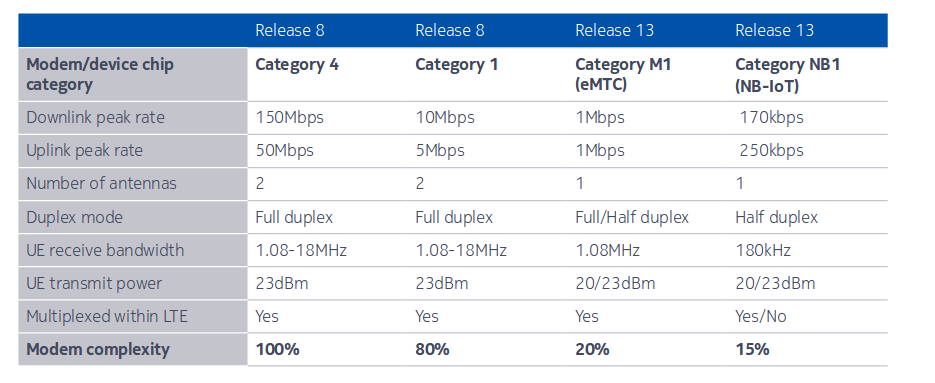
\includegraphics[width=\linewidth]{Images/Kategoriat.png}
    \caption{Taulukko päätelaitekategorioista \cite{nokiawhitepaper}.}
    \label{fig:kategoria}
\end{figure}

\textit{Release 12}:ssa \cite{release12} M2M-päätelaitteille esiteltiin \textit{Category 0}, jonka tarkoitus on vähentää päätelaitteiden kompleksisuutta ja energiankulutusta verrattuna \textit{Category 1}:een. \textit{Cat-0} laitekategorian lataus- ja lähetysnopeudet on laskettu 1 Mbps:iin, minkä lisäksi kategorian laitteet voivat viestiä vain yhdellä vastaanottoketjulla \cite{gsmawhitepaper}. Lisäksi vuorosuuntainen liikenne on laitteille sallittu taajuusjakoista kaksisuuntaisuutta käytettäessä. Tämän myötä aika-avaruudessa lomitetussa kaksisuuntaisessa liikenteessä ei enää tarvita erillistä suodatinta.

\textit{Cat-0}:n päätelaitteiden vastaanottokaistan leveys on kavennettu sekä lataus- että lähetyskaistalla 1,4 MHz:iin. Muutos mahdollistaa tehokkaamman AD-muunnoksen ja puskurin pienentämisen, minkä seurauksena laitteet pystyvät toimimaan hitaammalla prosessorilla ja muistilla \cite{nokiawhitepaper}. Kaventuneesta kaistanleveydestä huolimatta laitteet voivat toimia kaikilla LTE-järjestelmän käyttämillä kaistoilla aina 20 MHz:iin asti. Virrankulutuksen vähentämiseksi \textit{Release 12}:ssa päätelaitteiden maksimilähetystehoa pudotettiin myös 20 dBm:a.

Kuten aiemmin kappaleessa todettiin, \textit{Cat-0}:n laitteet toimivat 1,4 MHz:n kantoaallolla, joka vastaa kuutta fyysistä resurssilohkoa. Kategorian päätelaite, kuten mikä tahansa muu laite, kuuntelee aina kuutta keskimmäistä resurssilohkoa, joilta laite saa kontrolli-informaation \cite{nokiawhitepaper}. Kun laitteen on vuoro liikennöidä verkossa, sille osoitetaan yhdestä kuuteen peräkkäistä resurssilohkoa käytettävältä spektriltä. Laitteelle tarkoitettu kontrolli-informaatio ja data lomitetaan taajuustasossa ottamatta huomioon varhaisempien LTE-standardien kontrolli-informaatiota. Näin mahdollistetaan päätelaitteiden aikataulutus myös varhaisemmissa LTE-järjestelmissä.

\textit{Release 12}:ssa esiteltiin myös päätelaitteiden virransäästötila \cite{nokiawhitepaper}. Virransäästötilaa tukeva laite pyytää verkolta ajastimen verkkoon liittymisen tai paikannus (TAU) proseduurin aikana. \textit{Release 13}:ssa \cite{release13} julkaistiin \textit{Category M1}, jolla päätelaitteiden kompleksisuutta pyrittiin vähentämään vielä enemmän \cite{gsmawhitepaper}. Kategoria on tarkoitettu samantyyppisille sovelluksille kuin \textit{Cat-0}, ja tekniikka kulkee nimellä enhanced MTC (eMTC). Lisäksi samalla julkaistiin \textit{Category NB1} NB-IoT-verkkoteknologiaa hyödyntäville laitteille. 

\subsection{NB-IoT}

3GPP:n \textit{Release 13}:ssa esitelty kapeakaistainen esineiden internet eli NB-IoT (Narrowband IoT) on LTE-järjestelmän valmiiden toiminnallisuuksien päälle rakennettu IoT-laitteiden verkkoteknologia. Sen tavoitteena on mahdollistaa erittäin alhaisen kompleksisuuden IoT-laitteille tuki mobiiliverkossa, 20 dB:ä parempi sisätilojen kattavuus GPRS:een verrattuna, tuki yli 52 000:lle samaan aikaan kytketylle laitteelle, sekä yli kymmenen vuoden akunkesto 5 Wh akuille \cite{ratasuk2016overview}. Lisäksi NB-IoT-järjestelmän ei tulisi haitata samalla taajuuskaistalla toimivia, olemassa olevia mobiiliverkkojärjestelmiä.

NB-IoT tukee kolmea toimintatilaa. Se voi toimia itsenäisesti (stand-alone) hyödyntäen yhtä tai useampia GSM-kantoaaltoa, käyttäen LTE-järjestelmän kaistansisäisiä (in-band) resurssilohkoja tai LTE-järjestelmän kantoaallon suojakaistan (guard-band) sisäisiä, käyttämättömiä resurssilohkoja. Resurssilohkojen jakaminen LTE- ja NB-IoT-järjestelmien välillä mahdollistaa tehokkaamman taajuusspektrin käytön, minkä lisäksi molempien järjestelmien tuki voidaan saavuttaa samalla tukiaseman laitteistototeutuksella. GSM-kantoaaltoja käytettäessä NB-IoT pystyy hyödyntämään jo hyvin laajan kattavuuden maailmanlaajuisesti saanutta GSM-infrastruktuuria. \cite{ratasuk2016nb, ratasuk2016overview}

NB-IoT:n latauskaista on jaettu 15 kHz:n alikantoaaltoihin ja modulaatiomenetelmänä käytetään OFDMA:ta \cite{ratasuk2016nb}, mikä eroaa \textit{Release 8}:ssa määritellystä 20 Mhz:n kantoaallosta ja QPSK-, 16QAM- ja 64QAM-modulaatiomenetelmistä \cite{release8}. Tämä mahdollistaa kuuden fyysisen resurssilohkon lomittamisen yhteen resurssilohkoon ja NB-IoT:n toiminnan kaistansisäisesti. NB-IoT:n lähetyskaista tukee 3,75 kHz:n ja 15 kHz:n alikantoaaltoja yksisuuntaisissa lähetyksissä (single-tone transmission) \cite{ratasuk2016nb}. Kaksisuuntaisissa lähetyksissä (multi-tone transmission) tuki on 15 kHz:n alikantoaalloille ja SC-FDMA-modulaatiomenetelmälle.

Merkittävä muutos NB-IoT:ssä on neljän fyysisen kanavan karsiminen. NB-IoT:ssa käytössä ovat kanavat NPDCCH, NPDSCH, NPBCH, NPSS, NSSS, NPUSCH ja NPRACH, minkä johdosta alkuperäisestä LTE-standardin \textit{Release 8}:sta karsittujen PMCH, PCFICH, PDCCH ja PHICH kanavien sisältämä informaatio kuljetetaan jäljellä olevia kanavia pitkin \cite{ETSIts36211, harmaala}. Tämä mahdollistaa sen, että päätelaitteita voidaan yksinkertaistaa ja vähentää niiden virrankulutusta. Tämän lisäksi verkon resurssienkäyttö tehostuu \cite{ratasuk2016nb, harmaala}.

\clearpage
\section{LTE-standardin kehityksen tulevaisuuden näkymät}

\textit{Release 13}:n jälkeen 3GPP:n standardoinnin pääpaino siirtyi LTE:n kehityksestä 5G:n standardointiin ja tutkimiseen \cite{ericssonRelease14}. LTE-järjestelmien kehitys jatkuu taaksepäin yhteensopivien parannusten kehittämisellä olemassa olevalle radiospektrille, kun taas 5G:n kehitys keskittyy isompi taajuuksisen, varaamattoman radiospektrin ja RAN:n kehittämiseen. Kehitystyötä tehdään tiiviissä yhteistyössä, jotta LTE-järjestelmätkin pystyvät saavuttamaan tiukkoja 5G:n edellytyksiä. 3GPP on määritellyt omiin 5G-järjestelmän edellytyksiinsä parannetun mobiililaajakaistan (eMBB), mittavan koneiden välisen kommunikaation (mMTC) ja erittäin luotettavan vähälatenssisen kommunikaation (URLLC) \cite{hoymann2016lte}.

eMBB:n toteutuminen vaatii 5G-järjestelmältä kapasiteettia tukea kasvavaa viestiliikenteen määrää ja samalla sen tulee tarjota käyttäjille kaikkialla vähintään 10 Mbps nopeuden ja 20 Gbps:n huippudatansiirtonopeus. Tiheään rakennetut verkon tukiasemat, laajemman radiospektrin käyttö ja spektrinkäytön tehokkuuden parantaminen ovat välttämätön edellytys eMBB:n toteutumiselle \cite{hoymann2016lte}. Esimerkiksi tukiasemien sijoittaminen muun muassa lyhtypylväisiin ja lisensoimattoman radiospektrin hyödyntäminen ovat jo käytössä olevia menetelmiä yhteyden parantamiseksi.

mMTC:lla tarkoitetaan tukea vähäisen liikenteen ja pitkän akunkeston laitteille, kuten sensoreille ja vastaaville laitteille \cite{hoymann2016lte}. mMTC asettaa haasteita verkon kattavuudelle ja signaalinkäsittelylle. Tässä kandidaatintyössä kappaleessa 3 esitetyt LTE-M- ja NB-IoT-teknologiat osaltaan vastasivat jo mMTC:n asettamiin haasteisiin, mutta kehityksen on tarkoitus jatkua tulevissa 3GPP:n julkaisuissa.

URLLC:lla tarkoitetaan kommunikaatioyhteyden latenssin ja luotettavuuden parantamista. Luotettava ja matalan latenssin kommunikaatio mahdollistaa muun muassa uusien terveys-, turvallisuus- ja hallintapalveluiden toteuttamisen esineiden internetin avulla \cite{hoymann2016lte}. Esimerkiksi \textit{Release 14}:ssä esitelty älykäs liikennejärjestelmä (ITS) vaatii toimiakseen luotettavan LTE-kommunikaation \cite{ericssonITS}.

\subsection{Release 14}

LTE-järjestelmien kehitys jatkui \textit{Release 14}:ssä \cite{release14} latenssien vähentämisellä sekä lisensoimattoman spektriin, M2M-kommunikaatioon ja MIMO-tekniikkaan liittyvillä parannuksilla \cite{ericssonRelease14}. Latenssia on pienennetty mahdollistamalla lähetyskaistalla lähettäminen osalle laitteista ilman aikataulutuspyyntöjä \cite{hoymann2016lte}. Perinteisesti päätelaitteen täytyy pyytää tukiasemalta lupa datan lähettämiselle, joten muutoksella vältytään aikataulutuspyynnön ja lähetyskaistan myöntämisen aiheuttamalta viiveeltä ja round-trip-viiveajalta (kuva \ref{fig:URLLC}).

\begin{figure}[h!]
    \centering
    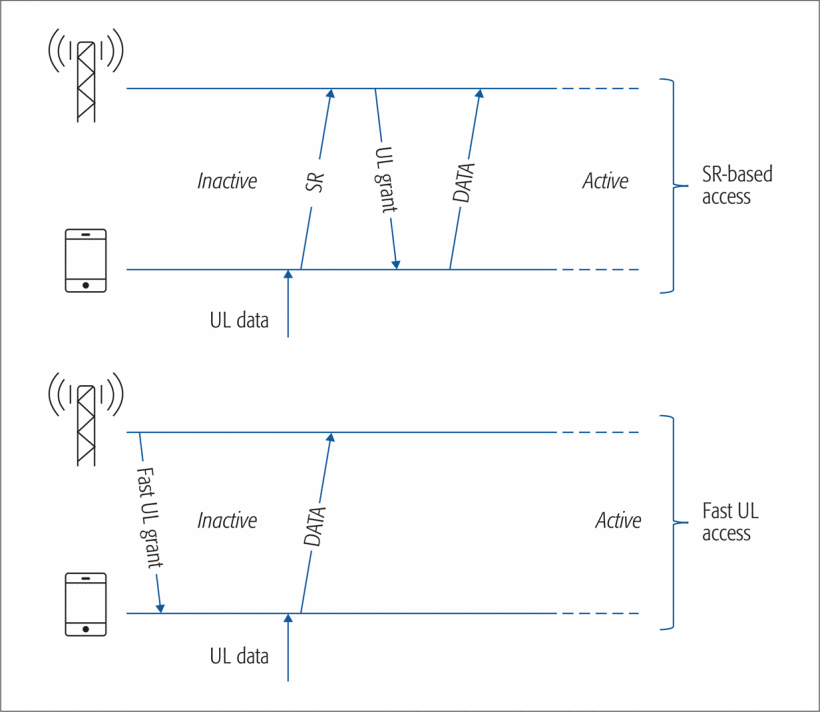
\includegraphics[scale=0.4]{Images/URLLC.png}
    \caption{Aikataulutuspohjainen yhteys (ylhäällä) ja nopean lähetyskaistan yhteys (alhaalla) \cite{hoymann2016lte}.}
    \label{fig:URLLC}
\end{figure}

NB-IoT koki myös parannuksia \textit{Release 14}:ssä ja \textit{Release 15}:ssä \cite{release15}. Päätelaitteen paikannusta parannettiin esittelemällä kolme paikannustapaa \textit{Release 13}:ssa esitellyn soluidentiteettipaikannuksen sijaan (CID) \cite{ratasuk2017enhancements}. Parannetussa E-CID-paikannuksessa hyödynnetään lähetys- ja vastaanottoaikojen aikaeroa sekä referenssisignaalin vastaanottotehoa ja -laatua \cite{hoglund2017overview}. OTDOA-paikannuksessa päätelaite mittaa latauslinkillä usealta lähettävältä tukiasemalta uuden paikannusreferenssisignaalin (NPRS) ToA-aikoja. Mittauksista muodostetaan geografisia hyberbolia, joiden risteyskohdassa päätelaitteen voidaan päätellä sijaitsevan \cite{hoglund2017overview}.

Uusi päätelaitekategoria \textit{Cat-NB2} esiteltiin tukemaan moninaisempia radioliikenneskenaarioita \cite{hoglund2017overview}. Uuden kategorian laitteet on tarkoitettu suotuisemmissa radio-olosuhteissa oleville laitteille. Kategorian laitteet pääsevät nopeampiin huippudatansiirtonopeuksiin 2536 bittiin kasvatetun TBS:n ja toisen HARQ-prosessiin tuen ansiosta. Lisäksi \textit{Release 14}:ssä paranneltiin tukiasemien monilähetystä, jonka avulla usean älykkään laitteen samanaikainen ohjelmistopäivitys on mahdollista. Lisäksi saatiin pienennettyä usealle laitteelle kommunikoinnin latenssia.

\subsection{Release 15}

5G-teknologian ensimmäisen vaiheen kehitys alkoi 3GPP:n \textit{Release 15} -standardissa, joka on valmistumassa syyskuussa 2018 \cite{release15}. Ensimmäisen 5G-radioverkon, 5G New Radion (5G-NR), standardin on tarkoitus olla valmis \textit{Release 16} -standardissa \cite{release16}. Joulukuussa 2017 3GPP:n kokouksessa Lissabonissa hyväksyttiin 5G-NR:n fyysinen kerros \cite{5GNRSpecs,TS38211}. 5G-NR käyttää LTE:n ja Wi-Fin tavoin OFDM-modulaatiota \cite{TS38211}, mikä tekee siitä ensimmäisen mobiiliverkon generaation, joka ei perustu uuteen aaltomuotoon.

\textit{Release 15}:ssä konetyyppisten laitteiden kommunikaatiota parannetaan pienentämällä latenssia ja virrankulutusta sekä lisäämällä tuki aikajakoiselle kaksisuuntaisuudelle \cite{ratasuk2017enhancements}. Aiemmissa LTE:n versioissa päätelaite on joutunut uusimaan pääinformaatiolähetyksen, jos pääinformaatiolähetys ja PDSCH-kanavalla kulkeva järjestelmäinformaatiolähetys 1 (SIB1) ylittävät ajallisesti SIB1:n uusimisjakson. Ongelma pyritään korjaamaan lisäämällä järjestelmäinformaatiolähetyksien toistoa muilla alikehyksillä ja kantoaalloilla sekä lisäämällä uusia laitteen herätysmekanismeja, jotka eivät tarvitse toimiakseen näitä lähetyksiä \cite{ratasuk2017enhancements}.

Päätelaitteiden virrankulutuksen pienentäminen on myös tärkeä tavoite \textit{Release 15}:ssä. Tyypillinen IoT-sovellus ei tarvitse aikataulutusta tukiasemalta kovinkaan usein, mutta laitteen täytyy olla tukiaseman tavoitettavissa järkevän pituisessa ajassa \cite{ratasuk2017enhancements}. Siksi päätelaite joutuu käyttämään suhteellisen paljon tehoa NPDCCH-kanavan monitorointiin. \textit{Release 15}:ssä on tarkoitus tutkia, voidaanko päätelaitteille saada aikaan merkittäviä virransäästöjä kehittämällä LTE:n paging-ominaisuutta, epäjatkuvaa vastaanottoa (DRX), tai hyödyntämällä uutta, helposti dekoodattavaa fyysistä kanavaa tai signaalia, jonka perusteella voidaan välttää turhaa NPDCCH- ja NPDSCH-kanavan dekoodaamista \cite{ratasuk2017enhancements}.

\subsection{LTE lisensoimattomalla spektrillä}

LTE-verkkojen nopeasti kasvava liikenteen määrä houkuttelee operoimaan LTE-järjestelmiä 5 GHz:n lisensoimattomalla radiospektrillä. Lisensoimattomalla spektrillä verkon kapasiteettia on halvempaa kasvattaa kuin lisensoidulla kaistalla. Tällä hetkellä kriittisin ongelma 5 GHz:n kaistan käyttämiselle on se, että samalla kaistalla toimii Wi-Fi-teknologia \cite{ismaiel2017survey}. Joidenkin tutkimusten mukaan samalla kaistalla toimivat teknologiat saattavat häiritä toisiaan ja heikentää molempien verkkojen toimintaa \cite{naik2018coexistence, ismaiel2017survey}.

Ensimmäinen lisensoimattomalla spektrillä toimiva LTE-teknologia, LTE Unlicensed (LTE-U), perustui LTE:n \textit{Release 12}:een. LTE-U-standardista kuitenkin puuttuu niin sanottu \textit{kuuntele ennen lähettämistä} -tekniikka (LBT). Sitä vaaditaan Euroopassa ja Japanissa radiotekniikoille, jotka käyttävät lisensoimatonta radiospektriä \cite{ismaiel2017survey}. 3GPP:n Release 13:ssa standardoitiin LTE-U:hun perustuva LTE-Licensed Assisted Access (LTE-LAA), johon kuului myös LBT-tekniikka. \textit{Release 13}:ssa esiteltiin myös LTE Wi-Fi Aggregation (LWA), joka mahdollistaa Wi-Fi-tukiasemien hyödyntämisen LTE-tekniikalle \cite{ismaiel2017survey}. LWA toimii siten, että osa LTE:n liikenteestä siirretään Wi-Fi:n kautta käyttäen CSMA-protokollaa.

\begin{figure}[h!]
    \centering
    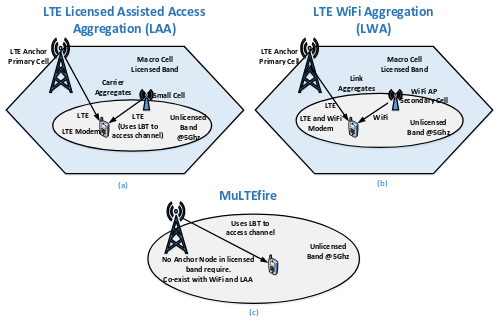
\includegraphics[scale=0.5]{Images/unlicensed.png}
    \caption{LTE lisensoimattomalla spektrillä \cite{ismaiel2017survey}.}
    \label{fig:unlicensed}
\end{figure}

MulteFire on MulteFire Alliancen kehittämä LTE-pohjainen tekniikka, joka toimii täysin lisensoimattomalla radiospektrillä. Se perustuu 3GPP:n \textit{Release 13}:ssa ja \textit{Release 14}:ssä esiteltyihin LAA- ja eLAA-tekniikoihin \cite{chambers2016multefire}, mutta eroaa näistä siten, että se ei tarvitse ankkuritukiasemaa lisensoidulta radiospektriltä (kuva \ref{fig:unlicensed}) \cite{ismaiel2017survey, multefire2015lte}. MulteFire hyödyntää LBT-tekniikkaa, joten se voi toimia samassa ympäristössä esimerkiksi Wi-Fi- ja LAA-järjestelmien kanssa. Koska MulteFire perustuu LTE-järjestelmään, se toimii 20 MHz:n alikaistoilla, joista se osaa eLAA:n tapaan dynaamisesti valita vähiten käytetyimmät kanavat \cite{chambers2016multefire}. Dynaaminen alikaistanvalinta vähentää muihin radiospektriä käyttäviin järjestelmiin aiheutuvia häiriöitä.

\begin{figure}[h!]
    \begin{minipage}{0.5\textwidth}
        \centering
        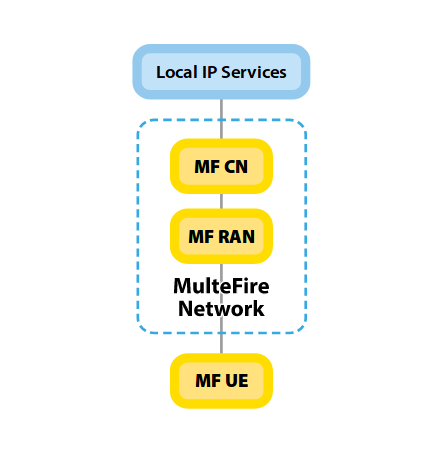
\includegraphics[width=0.5\linewidth]{Images/MF1.png}
        \caption{Itsenäinen toimintatila \cite{chambers2016multefire}.}
        \label{fig:MF1}
    \end{minipage}
    \begin{minipage}{0.5\textwidth}
        \centering
        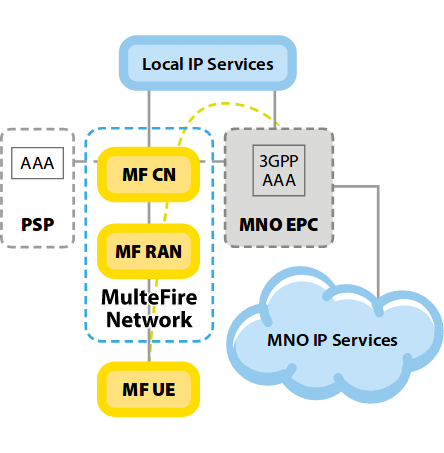
\includegraphics[width=0.5\linewidth]{Images/MF2.png}
        \caption{Itsenäinen verkko verkkovierailutuella ulkoisille mobiiliverkoille \cite{chambers2016multefire}.}
        \label{fig:MF2}
    \end{minipage}
\end{figure}

MulteFire tukee kolmea toimintatilaa. Itsenäisessä toimintatilassa (Kuva \ref{fig:MF1}) MulteFire tukiasemat muodostavat yksityisen ja omavaraisen verkon. Verkon laitteet eivät tarvitse omaa SIM-korttia, mutta verkosta löytyy tuki virtuaalisille tai yksityisille SIM-korteille \cite{chambers2016multefire}. Kuvan \ref{fig:MF2} verkko toimii muuten samoin kuin itsenäinen MulteFire-verkko, mutta verkko toimii myös neutraalina verkkovierailupalveluntarjoajana ulkoisten operaattorien verkkojen käyttäjille. Kolmannessa toimintatilassa MulteFiren verkko toimii osana operaattorin mobiiliverkkoa. Olemassa olevia SIM-kortteja käytetään verkkoon yhdistäessä. MulteFiren voi tukea kaikkia mahdollisia toimintatilojen kombinaatioita samanaikaisesti. Tämä on hyödyllistä esimerkiksi, kun yrityksen toimitiloissa erotetaan vierailijaverkot henkilökuntaverkoista.

\begin{figure}[h!]
    \centering
    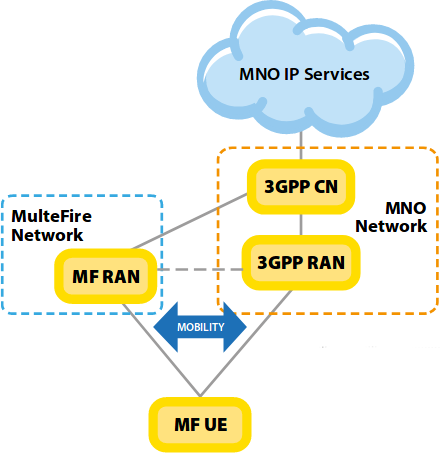
\includegraphics[scale=0.25]{Images/MF3.png}
    \caption{Ulkoisiin mobiiliverkkoihin tiukasti integroitu verkko \cite{chambers2016multefire}.}
    \label{fig:MF3}
\end{figure}

MulteFiren julkaisuversio 1.1 on valmistumassa kesäkuussa 2018 \cite{multefire11}. Julkaisussa MulteFirea on optimoitu IoT-laitteiden käyttöön. Lisäksi LTE-järjestelmistä tutut eMTC- ja NB-IoT-tekniikat on lisätty MulteFiren standardiin. NB-IoT-laitteet voivat \textit{MulteFire 1.1}:ssä toimia alle 1 GHz:n, 1,9 GHz:n ja 2.4 GHz:n radiospektrillä. eMTC-laitteet voivat toimia näiden lisäksi vielä 3.5 GHz:n radiospektrillä. Päivityksen myötä \textit{MulteFire 1.1} vastaa pitkälti LTE-standardin \textit{Release 14}:ä. MulteFiren kehitys jatkuu rinnakkaisena LTE:n kehityksen kanssa.

\clearpage
\section{Yhteenveto}

Tässä kandidaatintyössä selvitettiin, miten LTE-järjestelmää on kehitetty tukemaan paremmin esineiden internetin ja laitteiden välisen kommunikaation asettamia vaatimuksia. LTE-standardin kehitystä tarkasteltiin jo valmistuneiden ja käyttöönotettujen \textit{Release 12}- ja \textit{Release 13} -julkaisujen kehitystyöhön ja kehysrakenteeseen tutustumalla. Työn neljännessä kappaleessa tutustuttiin valmistuneeseen \textit{Release 14}:ään ja valmisteilla olevaan \textit{Release 15}:een. Tämän lisäksi työssä tutustuttiin, miten LTE-järjestelmän ja siihen perustuvassa MulteFire-järjestelmän kehitystyössä on alettu hyödyntää lisensoimatonta radiospektriä.

Esineiden internetillä tarkoitetaan  esineiden muodostamaa verkkoa, jossa laitteet keräävät ja lähettävät tietoa toisilleen. Esineiden internetin myötä internetiin kytkettyjen laitteiden määrän uskotaan kasvavan 50 miljardiin laitteeseen vuoteen 2020 mennessä. Näistä laitteista noin 7 miljardia on liitetty internetiin hyödyntäen niin sanottuja LPWA-verkkoja.

Esineiden internetin verkkoliikenne muodostuu merkittävissä määrin koneiden välisestä kommunikaatiosta, mikä eroaa huomattavasti ihmisten välisestä kommunikaatiosta. Kommunikaatio koostuu usein pienistä datalähetyksistä, ja sen täytyy olla luotettavaa. Laitteille on tärkeää, että verkkoon yhdistäminen ei kuluta liikaa akunkestoa, sillä laitteiden akun vaihtaminen on kallis toimenpide. Verkon täytyy myös olla maantieteellisesti kattava ja tukea suurta määrä päätelaitteita ilman verkon ruuhkautumista. Samalla laitteiden ja verkon kehityskustannusten tulee olla edullisia.

Alun perin ihmisten väliseen kommunikaatioon kehitettyä LTE-standardia on kehitetty tukemaan paremmin esineiden internetin tarpeita. Alkuperäisessä \textit{Release 8}:ssa esiteltyjen päätelaitekategorioiden rinnalle kehitettiin \textit{Release 12}:ssa kategoria \textit{Category 0}, jossa päätelaitteita yksinkertaistettiin ja samalla pienennettiin nopeutta. \textit{Release 13}:ssa esiteltiin kapeakaistainen esineiden internet ja sen päätelaitekategoria \textit{Category NB1}. Sen on tarkoitus mahdollistaa tuki erittäin yksinkertaisille IoT-laitteille. Yksinkertaistus on toteutettu karsimalla fyysisen kerroksen kanavia ja lomittamalla kuusi fyysistä resurssilohkoa yhteen resurssilohkoon.

\textit{Release 13}:n jälkeen LTE-standardin kehitys siirtyi 5G-standardin kehittämiseen ja tutkimiseen. Kehitystyössä keskitytään parantamaan verkon kapasiteettia ja nopeuksia, tukemaan paremmin vähäisen liikenteen ja pitkän akunkeston laitteita sekä kommunikaatioyhteyden latenssin pienentämiseen ja luotettavuuden parantamiseen. \textit{Release 14}:ssä latenssia pienennettiin ja NB-IoT-teknologiaa kehitettiin. Lisäksi julkaisussa esiteltiin uusi päätelaitekategoria \textit{Category NB2} tukemaan moninaisempia radioliikenneskenaarioita. \textit{Release 15}:n kehitystyö on vielä keväällä 2018 kesken, mutta julkaisussa on uuden 5G-radioverkon lisäksi tarkoitus parantaa edelleen IoT-laitteiden latenssia ja virrankulutusta.

LTE-verkkojen kapasiteetin parantamiseksi on myös LTE-standardia kehitetty toimimaan 5 GHz:n lisensoimattomalla radiospektrillä. Tällaisia teknologioita ovat muun muassa \textit{Release 12}:een perustuva LTE Unlicensed, LTE Licensed Assisted Access ja Wi-Fi-tukiasemien hyödyntämiseen perustuva LTE Wi-Fi Aggregation. Nämä teknologiat eivät kuitenkaan toimi täysin lisensoimattomalla radiospektrillä, vaan vaativat operaattorin ankkuriaseman lisensoidulta spektriltä. Täysin lisensoimattomalla spektrillä kykenee toimimaan MulteFire-teknologia, jonka kesäkuussa 2018 valmistuva versio 1.1 perustuu LTE:n \textit{Release 14}:ään. MulteFire toimii integroituna operaattorin ulkoisiin verkkoihin tai omana itsenäisenä verkkonaan. Itsenäinen MulteFire-verkko tukee myös verkkovierailua muille verkoille.

%\section{Summary}

\clearpage
%% \phantomsection varmistaa, että hyperref-paketti latoo hypertekstilinkit
%% oikein.
%% The \phantomsection command is nessesary for hyperref to jump to the 
%% correct page, in other words it puts a hyper marker on the page.
\phantomsection{}

\thesisbibliography
\printbibliography

\clearpage
%% Lisää tekstin "Liitteet" sisällysluetteloon
%%
%% Adds the word "Appendices" to the table of contents
%\addtocontents{toc}{\protect\contentsline{section}{Liiteet}{}{appendix}}
%\addtocontents{toc}{\protect\contentsline{section}{Appendices}{}{appendix}}

%\section{Esimerkki liitteestä\label{LiiteA}}
%% Liitteiden kaavat, taulukot ja kuvat numeroidaan omana kokonaisuutenaan
%%
%% Equations, tables and figures have their own numbering in Appendices
%\renewcommand{\theequation}{A\arabic{equation}}
%\setcounter{equation}{0}  
%\renewcommand{\thefigure}{A\arabic{figure}}
%\setcounter{figure}{0}
%\renewcommand{\thetable}{A\arabic{table}}
%\setcounter{table}{0}

%Liitteet eivät ole opinnäytteen kannalta välttämättömiä ja opinnäytteen tekijän on kirjoittamaan ryhtyessään hyvä ajatella pärjäävänsä ilman liitteitä.Kokemattomat kirjoittajat, jotka ovat huolissaantekstiosan pituudesta, paisuttavat turhan helposti liitteitä pitääkseen tekstiosan pituuden annetuissa rajoissa.Tällä tavalla ei synny hyvää opinnäytettä.   

%Liite on itsenäinen kokonaisuus, vaikka se täydentääkin tekstiosaa.Liite ei siten ole pelkkä listaus, kuva tai taulukko, vaan liitteessä selitetään aina sisällön laatu ja tarkoitus. 

%Liitteeseen voi laittaa esimerkiksi listauksia. Alla on listausesimerkki tämän liitteen luomisesta. 

%% Verbatim-ympäristö ei muotoile tai tavuta tekstiä. Fontti on monospace.
%% Verbatim-ympäristön sisällä annettuja komentoja ei LaTeX käsittele. 
%% Vasta \end{verbatim}-komennon jälkeen jatketaan käsittelyä.

\end{document}